% !TEX root = ../main.tex
\section{Results}

We report the reproduced findings of the full experiment grid (18 landbases $\times$ 4 discount rates $\times$ 6 harvest-flow policies; 432 sequential-replanning simulations). Per the framing of this paper, these reproduce and refine \citet{daugherty1991credibility}'s findings on the real Umpqua FORPLAN case study; they are presented with their fidelity caveats in Section 5. Every number below is regenerated by the repository's tracked experiment entry point; the per-cell simulation records are the tracked benchmark record (\texttt{results/experiments/}), summarized with figures and tables in the curated supplement (\texttt{supplementary/02-core-grid.md}).

\textbf{The harvest-flow constraint is the operative link.} Dynamic inconsistency is pervasive under the harvest-flow policies but largely absent without one. Across the grid, 73\% of the flow-constrained cells (NDY, bounded decline, and bounded deviation) exhibit inconsistency by the divergence metric (equation~\eqref{eq:metric}), against 38\% of the no-harvest-flow (NHF) control cells -- and the NHF divergence is concentrated at the lowest discount rates (0--2\%), where the objective is nearly indifferent to timing; at 4--6\% the no-flow control is consistent (Section 5). In all flow-constrained cells the first-period decision is consistent -- the divergence is in the plan's tail, exactly as the theory predicts. Where a model links periods only through a harvest-flow constraint, its projected harvest trajectory is a property of a plan that sequential re-optimization will not follow.

\textbf{The declining non-declining yield.} On the all-mature landbase 1, the divergence between announcement and delivery is stark (Figure~\ref{fig:ndy}). The open-loop non-declining-yield plan projects a smooth, credible-looking level harvest flow; the realized replanned trajectory is revised downward over most of the horizon as each successive planner inherits the depleted forest and re-solves. This is the ``declining non-declining yield'' of \citet[pp.~331--332]{gunn2007models}: the promised non-declining flow declines precisely because each successive planner declines to honour it.

\begin{figure}[t]
\centering
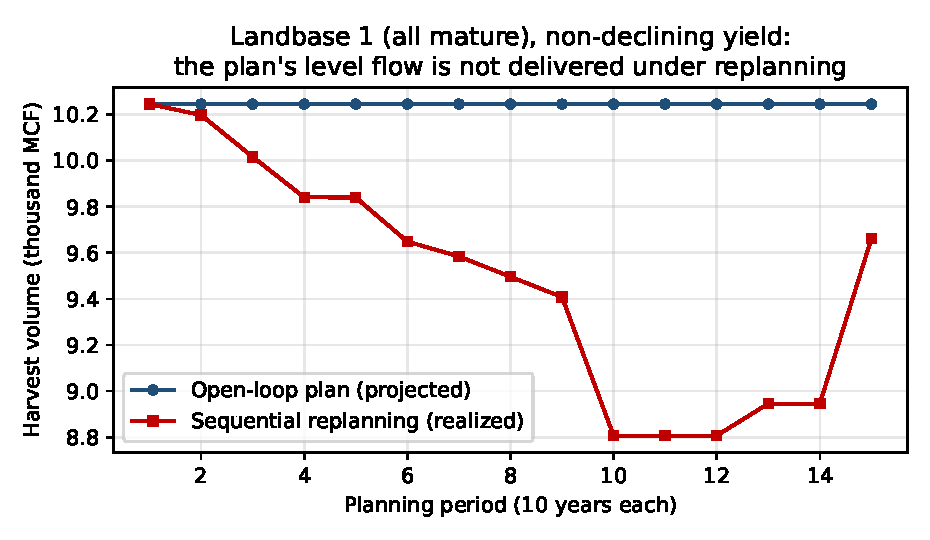
\includegraphics[width=\textwidth]{figures/fig_declining_ndy.pdf}
\caption{The declining non-declining yield on the all-mature landbase 1 under the non-declining-yield (NDY) harvest-flow policy at a 4\% discount rate. The open-loop plan projects a level, non-declining harvest flow; the realized sequential-replanning trajectory is revised downward over most of the horizon. Full provenance and the per-cell simulation records: \texttt{results/experiments/grid\_trajectories.csv}; supplement \texttt{supplementary/02-core-grid.md}.}
\label{fig:ndy}
\end{figure}

\textbf{Occurrence at every discount rate; magnitude is rate-dependent.} Inconsistency occurs at every discount rate in the grid (the flow-constrained occurrence rate is 100\% at 0\% and 47--86\% at 2--6\%), consistent with the thesis's analytical result that, because the discount factor is uniform across periods, it drops out of the consistency requirements \citep[ch.~3, p.~58--59]{daugherty1991credibility} -- the phenomenon does not require a particular rate. The \emph{magnitude} is rate-dependent: on landbase 1 under NDY, the mean relative divergence and the total-volume shortfall are markedly larger at a 0\% rate (where the objective is indifferent to timing) than at 2--6\%. We return to this nuance in the Discussion, because it refines -- rather than contradicts -- the naive account of the phenomenon.

\textbf{The divergence is genuine inconsistency, not an artifact of alternate optima.} Because LP optima can be non-unique, a divergence between the projected and realized trajectories could in principle reflect a different member of an optimal set rather than a plan that will not be followed. The objective-gap diagnostic (Section 3.3) rules this out: it re-solves each subproblem freely and again with the period-1 harvest held to the announced plan's value, and compares the objectives. On landbase 1 under NDY, the announced plan's tail is strictly suboptimal or outright infeasible from the realized state in 13--14 of 15 replan periods at every discount rate -- the re-solving planner strictly improves on, or cannot even implement, the announced tail. Under the no-flow control, by contrast, the announced tail remains optimal at every period at 4--6\% (and largely optimal at 0\%, where the flat objective admits alternate optima). The inconsistency is therefore a property of the flow-constrained plan, not of solver tie-breaking.

\textbf{Effect of the harvest-flow policy.} The strictness and form of the flow constraint shape the inconsistency. The non-declining-yield policy -- permitting no decrease -- produces the most frequent divergence (occurrence 86\%, the highest of the flow policies), and the magnitude of the divergence varies by policy and landbase (Table~\ref{tab:grid}). At the base and higher discount rates (4--6\%) the no-flow control is consistent (0\% occurrence), confirming the flow constraint as the operative between-period link; at the lowest rates (0--2\%) the no-flow control also diverges, which we attribute to timing-indifference (a near-flat objective admits near-tie optima that the re-solver resolves differently) rather than genuine inconsistency -- the objective-gap diagnostic (Section 3.3) confirms the no-flow tail remains optimal there.

\textbf{Role of disequilibrium structure.} The inconsistency occurs across all eighteen initial forest conditions (flow-constrained occurrence 50--100\% by landbase), and is most pronounced in magnitude on the disequilibrium structures: the all-mature and area-control-derived landbases, which place a pulse of immediately harvestable, financially over-mature volume in front of a regulated future that cannot sustain it. The CM-CE ecoclass is negatively valued -- its harvest cost exceeds its timber value -- and such strata enter the open-loop solutions as \emph{inconsistent variables}: area allocations whose only function is to relax the binding flow constraint in the plan and that the re-solving planner subsequently abandons.

\begin{table}[h]
\centering
\small
\caption{Experiment-grid summary: factors, levels, occurrence of dynamic inconsistency (share of cells exceeding the 5\% divergence tolerance), and mean magnitude (symmetric relative deviation, equation~\eqref{eq:metric}), over the full grid (432 cells). Full per-cell simulation records: \texttt{results/experiments/grid.csv}; per-landbase detail in \texttt{supplementary/04-landbases.md}.}
\label{tab:grid}
\begin{tabular}{@{}llcc@{}}
\toprule
Factor & Levels & Occurrence & Mean magnitude \\
\midrule
Harvest-flow policy & NDY, $-10\%$, $-20\%$, $\pm10\%$, $\pm20\%$ & 58--86\% & 0.10--0.13 \\
\quad (control) & NHF (no harvest flow) & 38\% & 0.13 \\
Discount rate & 0\%, 2\%, 4\%, 6\% & 100\% / 47--86\% & rate-dependent \\
Initial forest condition & 18 landbases (Table 5.5) & 50--100\% & 0.08--0.23 \\
\bottomrule
\end{tabular}
\end{table}

\subsection{Extension results: four mitigation tests}

\textbf{E1: declining discount rates make it worse, via a second channel.} Replacing the constant rate with declining schedules (linear or inverse-j) raises flow-constrained occurrence to 98--100\% (vs.\ 47--86\% at constant 2--6\%) and mean magnitude to 0.16--0.20 (vs.\ 0.07--0.11): weighting the far future more heavily does not mitigate the phenomenon (Fig.~\ref{fig:e1}, Table~\ref{tab:extensions}). The separation comes from the no-flow control: under constant 4--6\% rates it is consistent (occurrence 0\%), but under every declining path it diverges at 100\% occurrence, and the objective-gap diagnostic shows the announced tails genuinely strictly suboptimal or infeasible (strictly suboptimal in 30--61\% of tail periods; infeasible in 7--14\%). With no inter-period constraint present, this is a pure preference-level (Strotz) inconsistency channel: each replanning planner re-applies the declining path from her own present and is therefore more impatient about her near term than the time-zero planner was about the same calendar period. Declining-rate schedules thus not only fail to repair the structural inconsistency -- they add a second, independent channel that operates even where the structural one is absent.

\textbf{E2: a calibrated max-harvest cap eliminates it.} Under the cap-search policy the inconsistency disappears everywhere: all 72 cells converge, and occurrence is 0\% at every discount rate (mean divergence 0.004, grid maximum 0.025 -- all below the 5\% tolerance). The objective-gap diagnostic confirms genuine consistency rather than tie-breaking: 96\% of replan periods leave the announced tail optimal (residual suboptimal/infeasible shares 3\%/0.2\%, noise level). On landbase 1 at 4\%, the calibrated even-flow level is about 9,400 MCF/period -- roughly 8\% below the NDY plan's announced 10,250 MCF/period that sequential replanning will not deliver (Fig.~\ref{fig:e2}). The cap search prices the credibility of the flow promise: the gap between the announced NDY level and the calibrated level is the allowable-cut effect made operational.

\textbf{E3: denominating the flow in dollars makes it worse -- and the filler is the tell, not the fuel.} Under revenue-denominated flow policies, flow-constrained occurrence rises to 99\% (vs.\ 73\% volume-denominated) and mean magnitude roughly doubles (0.16 vs.\ 0.12). The mechanism test is decisive: under volume NDY the open-loop plan schedules negatively valued CM-CE harvest equal to 2.5--3.5\% of projected volume on landbase 1 (the inconsistent-variable filler); under revenue NDY the projected CM-CE harvest is exactly zero -- the filler channel is structurally disabled -- yet the plan is still not followed (indeed, the revenue-NDY plan front-loads harder, with period-1 realized harvest about 30\% above the volume-NDY case). The negatively valued strata are therefore an observable marker of the inconsistency, not its cause; the fuel is the flow link interacting with the disequilibrium state, operating through the positive-value strata alone when the filler is unavailable. (Plumbing validation: the no-flow control is identical under both denominations.)

\textbf{E4: the constraint's shape is not the margin -- the anchoring institution is.} Under the within-plan institution, rolling-mean NDY is indistinguishable from pointwise NDY (occurrence 89\% vs.\ 86\%; magnitude 0.10) -- smoothing the reference level changes nothing. Under the realized-history institution, occurrence falls to 69\% and magnitude to 0.072: binding the future planner to what actually happened mitigates the divergence. But the floor then frequently cannot be sustained from the depleted realized state -- in 21\% of replan periods (up to 32\% at 6\%) the policy must relax, the declining non-declining yield surfacing as recorded infeasibility rather than silent abandonment. Both readings are defensible models of planning practice; the contrast makes the replanning institution itself a result, upgrading what was a robustness note in the core design.

\begin{table}[t]
\centering
\small
\caption{Extension-grid summary. Occurrence and mean magnitude (symmetric relative deviation, equation~\eqref{eq:metric}) over each extension grid; the control is the matched core-grid quantity. Full per-cell records and analyses: supplement \texttt{supplementary/05}--\texttt{08}.}
\label{tab:extensions}
\begin{tabular}{@{}p{5.6cm}cccc@{}}
\toprule
Extension (grid) & Cells & Occurrence & Mean magnitude & Verdict \\
\midrule
E1 declining discount paths (control: constant 2--6\%) & 432 & 0.98--1.00 (0.47--0.86) & 0.16--0.20 (0.07--0.11) & worsens \\
E2 calibrated max-harvest cap (control: NDY) & 72 & 0.00 (0.86) & 0.004 (0.10) & eliminates \\
E3 revenue-denominated flow (control: volume) & 864 & 0.99 (0.73) & 0.16 (0.12) & worsens \\
E4 rolling-mean NDY, within-plan (control: NDY) & 144 & 0.89 (0.86) & 0.10 (0.10) & no effect \\
E4 rolling-mean NDY, realized-history & 144 & 0.69 & 0.07 & mitigates \\
\bottomrule
\end{tabular}
\end{table}

\begin{figure}[t]
\centering
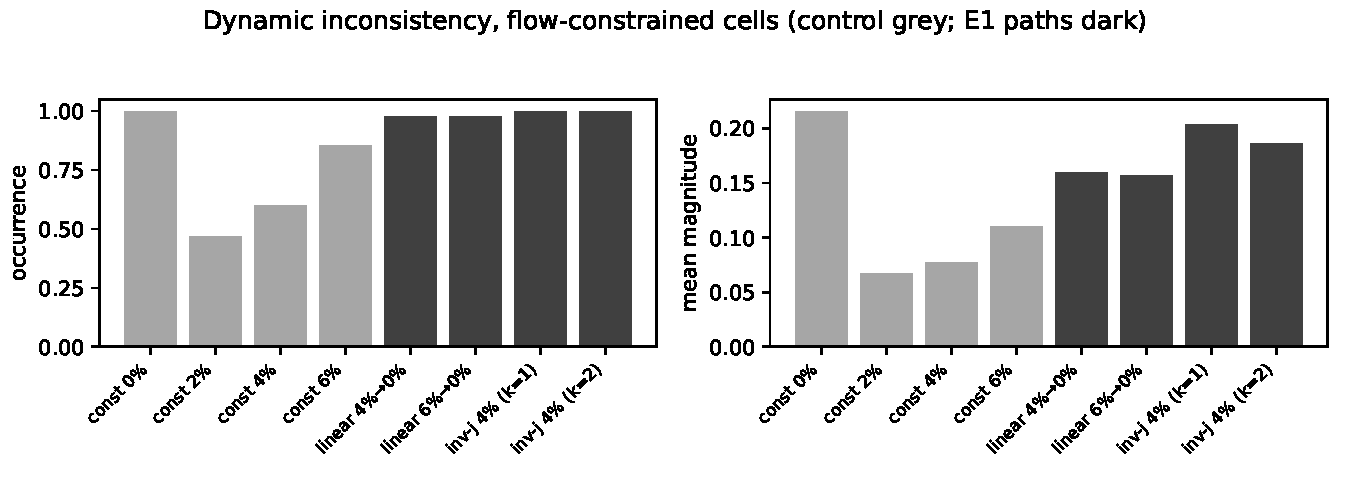
\includegraphics[width=\textwidth]{figures/fig_e1_occurrence_magnitude.pdf}
\caption{Dynamic inconsistency by discount scheme (flow-constrained cells): the constant-rate controls (grey) vs the declining-rate E1 paths (dark). Declining rates raise occurrence to 98--100\% and magnitude toward the 0\%-rate level. Regenerated from the tracked records; supplement \texttt{supplementary/05}.}
\label{fig:e1}
\end{figure}

\begin{figure}[t]
\centering
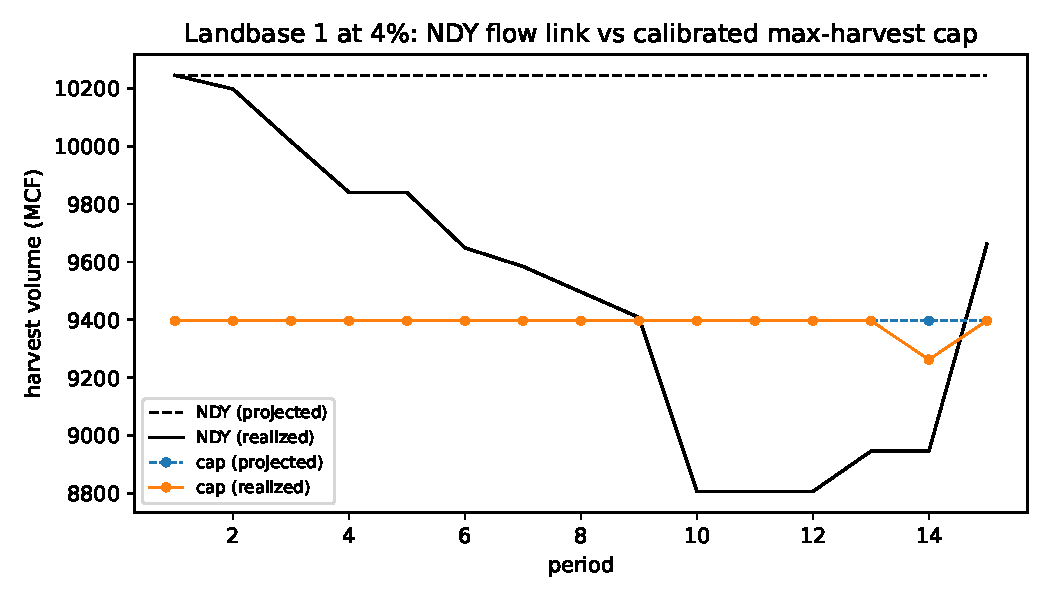
\includegraphics[width=0.7\textwidth]{figures/fig_e2_ndy_vs_cap.pdf}
\caption{Landbase 1 at 4\%: the NDY open-loop plan's level flow (dashed) and its declining realized trajectory (black) vs the calibrated max-harvest cap (orange), whose projected level the realized trajectory delivers. Regenerated from the tracked records; supplement \texttt{supplementary/06}.}
\label{fig:e2}
\end{figure}
